\section{Extraction of Compton Form Factors}\label{sec_cff}
The three sets of projected asymmetries (BSA from \cite{proposal}, shown in Fig.~\ref{fig_bsa}, TSA and DSA from this work, Figs.~\ref{fig_tsa_100_50_FT} and \ref{fig_dsa_100_50_FT}, respectively) for all kinematic bins were processed using the fitting procedure described in Section ~\ref{sec_michel_fits} to extract the Compton Form Factors of the neutron.  
In the adopted version of the fitter code, $\tilde{E}_{Im}(n)$ is set to zero, as $\tilde{E}(n)$ is assumed to be purely real - it is parametrized in the VGG model by the pion pole $(1/(t-m^2_{\pi}))$. Thus, seven out of the eight real and imaginary parts of the CFFs are left as free parameters in the fit. A loose bound on the parameters is also applied, limiting them within the interval given by $\pm 5 \cdot {\rm VGG}$, where "VGG" stands for the prediction of the VGG model for the value of the CFF.

%The results for the 7 neutron CFFs are shown in Figs.~\ref{cff_him}-\ref{cff_etre}, as a function of $-t$, and for each bin in $Q^2$ and $x_B$. The points are the CFFs resulting from the fits, and their error bars reflect both the statistical precision of the fitted observables and their sensitivity to that particular CFFs. Only results for which the error bars are non zero, and therefore the fits have properly converged for that CFF, are included here. For comparison, three kinds of scenarios are shown: the blue points points show the CFFs that can be extracted with 100 days of beamtime, and using the FT for the 50 required by this extension; the black points show the CFFs that can be extracted with 100 days of beamtime, and without using the FT; the red points show the CFFs that can be extracted with only the already approved 50 days of beam time of Run-Group Cb. 

The results for the 7 neutron CFFs are shown in Figs.~\ref{cff_him}-\ref{cff_etre}, as a function of $-t$, and for each bin in $Q^2$ and $x_B$. The points are the CFFs resulting from the fits, and their error bars reflect both the statistical precision of the fitted observables and their sensitivity to that particular CFFs. Only results for which the error bars are non zero, and therefore the fits have properly converged for that CFF, are included here. For comparison, three kinds of scenarios are shown: the blue points points show the CFFs that can be extracted with the proposed extended run group, while the red points show the CFFs that can be extracted with only the already approved 50 days of beam time of Run-Group Cb. 

The CFFs which will be obtained with more precision and for most of the kinematic points that will be covered by the proposed experiment are $H_{Im}(n)$ and $E_{Im}(n)$. This is to be expected, since the TSA and the BSA are most sensitive to these two CFFs. $H_{Im}(n)$ will benefit the most of the run-time extension as it is the CFF accessed thanks to the TSA. 
A quite good sensitivity to $\tilde{E}_{Re}(n)$ seems possible in a wide kinematics range. $\tilde{H}_{Re}(n)$ will also be obtained in most of the kinematic bins, thanks to the peculiar sensitivity of the DSA for this CFF. 
$\tilde{H}_{Im}(n)$ will be well extracted only in the low $Q^2$-$x_B$ kinematics. Finally, it appears that these data will not be able to provide much information on $E_{Re}(n)$.
The addition of the 60 extra days required by this experiment improves considerably both the statistics and the amount of bins for which the CFF fits converge, especially for $H_{Im}(n)$, but also for $\tilde{H}_{Im}(n)$ and $\tilde{E}_{Re}(n)$. $E_{Im}(n)$ appears to be less affected by the variations of statistics for the polarized-target data because the observable that has the most sensitivity to it is the BSA, measured on unpolarized deuterium. However, even for $E_{Im}(n)$ in some kinematics the extension will be beficial, allowing to retrieve CFFs for which otherwise the fits would not converge. 
The inclusion of the Foward Tagger improves the precision of the CFFs at low $-t$ and low $x_B$, for the high-$Q^2$ bins, mainly. 
\begin{sidewaysfigure}  
\begin{center}
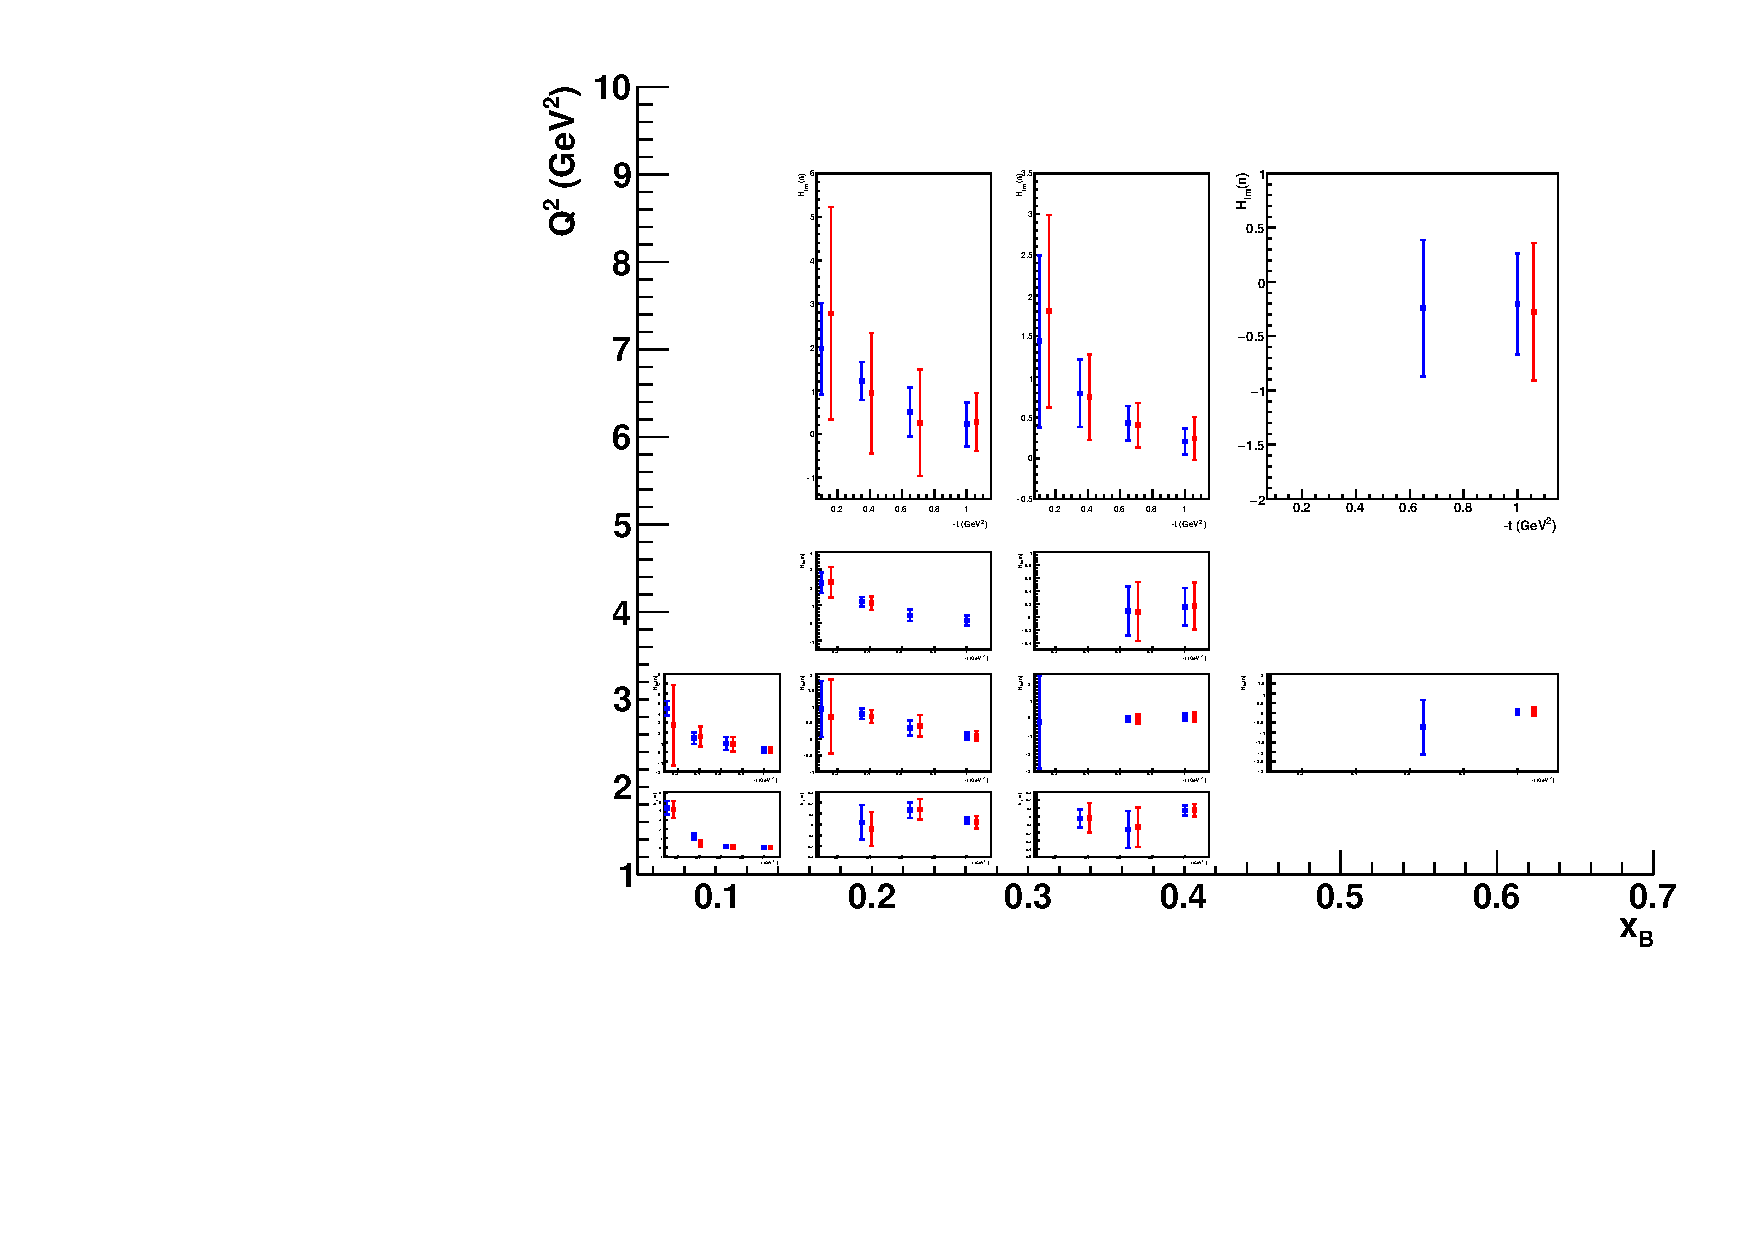
\includegraphics[width=200mm]{mixed_CFF/100/mixed/CFF_him_compare3.pdf}
\caption[$H_{Im}(n)$ as a function of $-t$]
{$H_{Im}(n)$ as a function of $-t$, for each bin in $Q^2$ and $x_B$. The blue points are obtained with the proposed run-group extension. The red points are obtained with the existing 50 days of Run Group Cb.}\label{cff_him}
\end{center}
\end{sidewaysfigure}

\begin{sidewaysfigure}  
\begin{center}
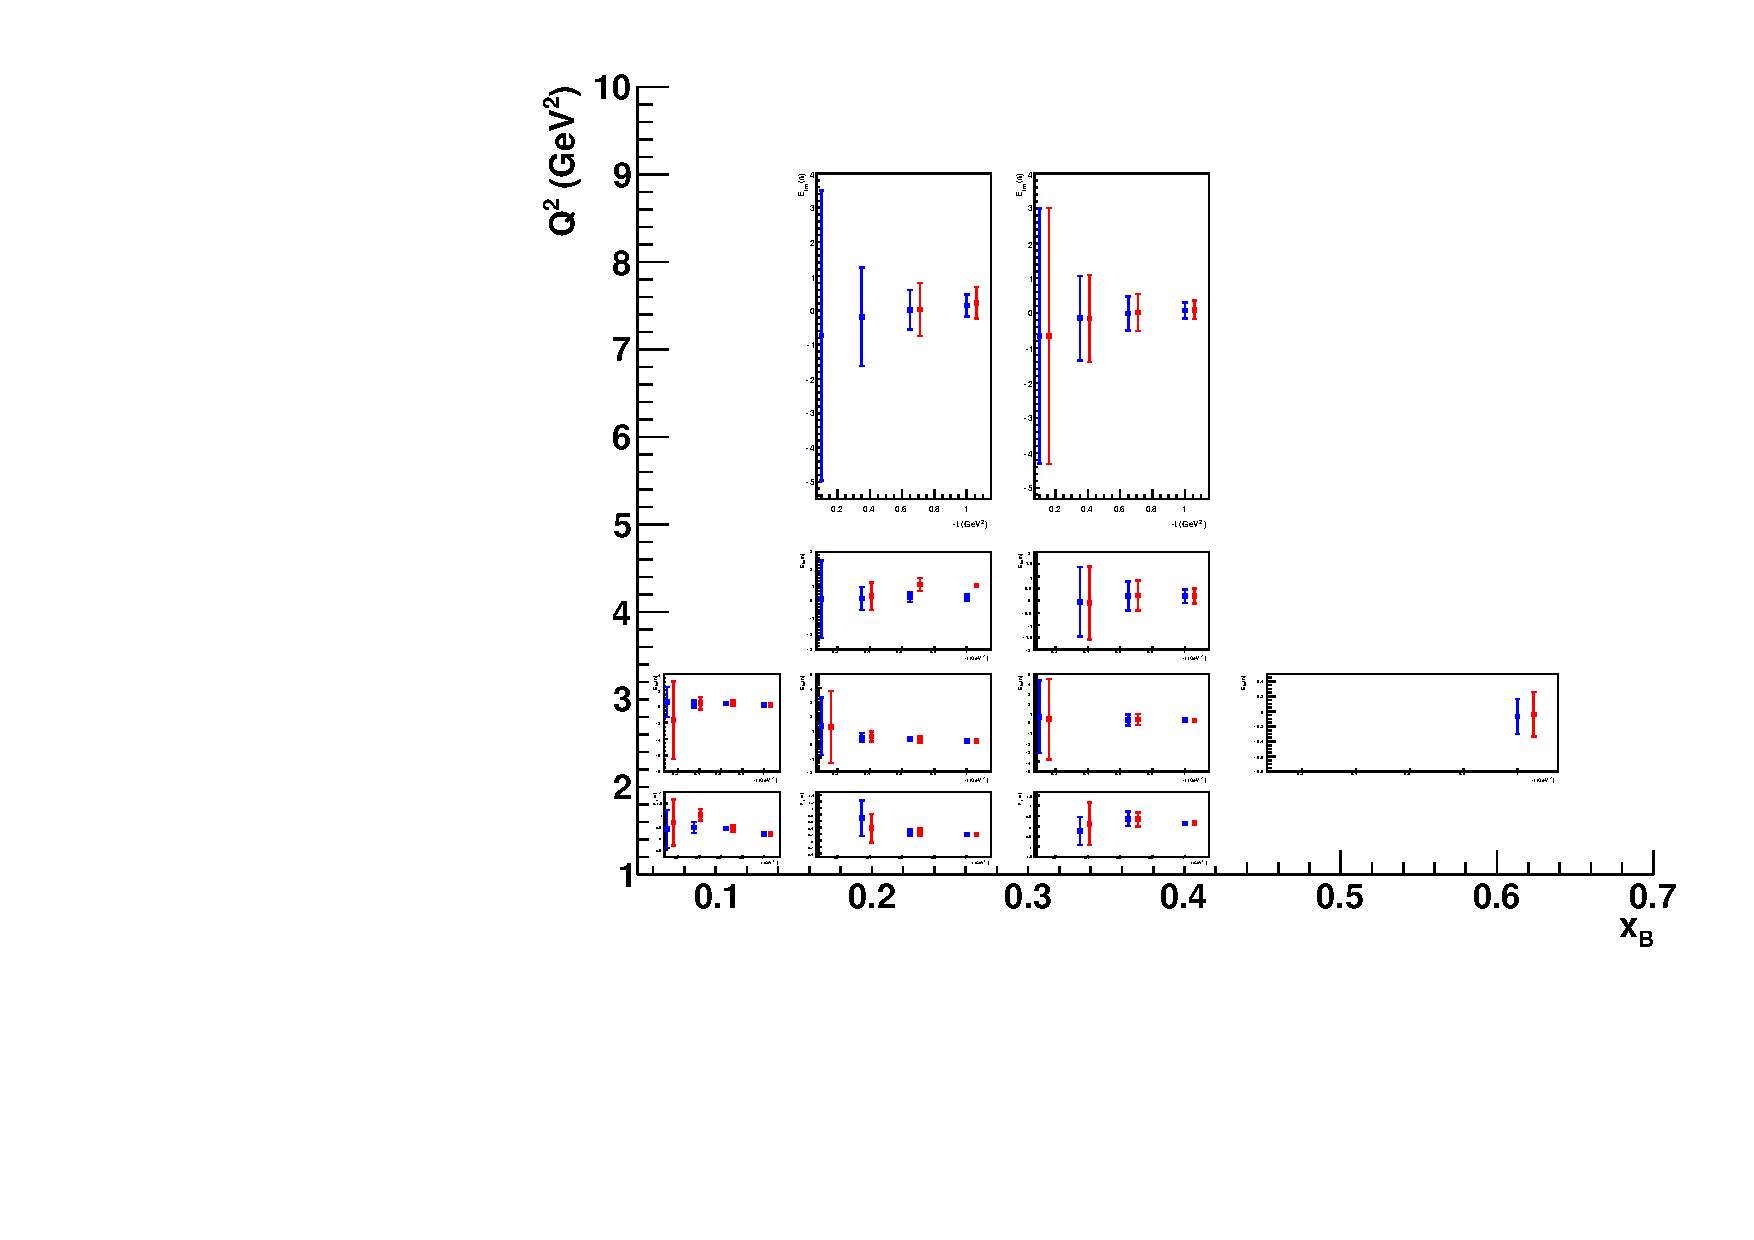
\includegraphics[width=200mm]{mixed_CFF/100/mixed/CFF_eim_compare3.pdf}
\caption[$E_{Im}(n)$ as a function of $-t$]
{$E_{Im}(n)$ as a function of $-t$, for each bin in $Q^2$ and $x_B$. The blue points are obtained with the proposed run-group extension. The red points are obtained with the existing 50 days of Run Group Cb.}\label{cff_eim}
\end{center}
\end{sidewaysfigure}

\begin{sidewaysfigure}  
\begin{center}
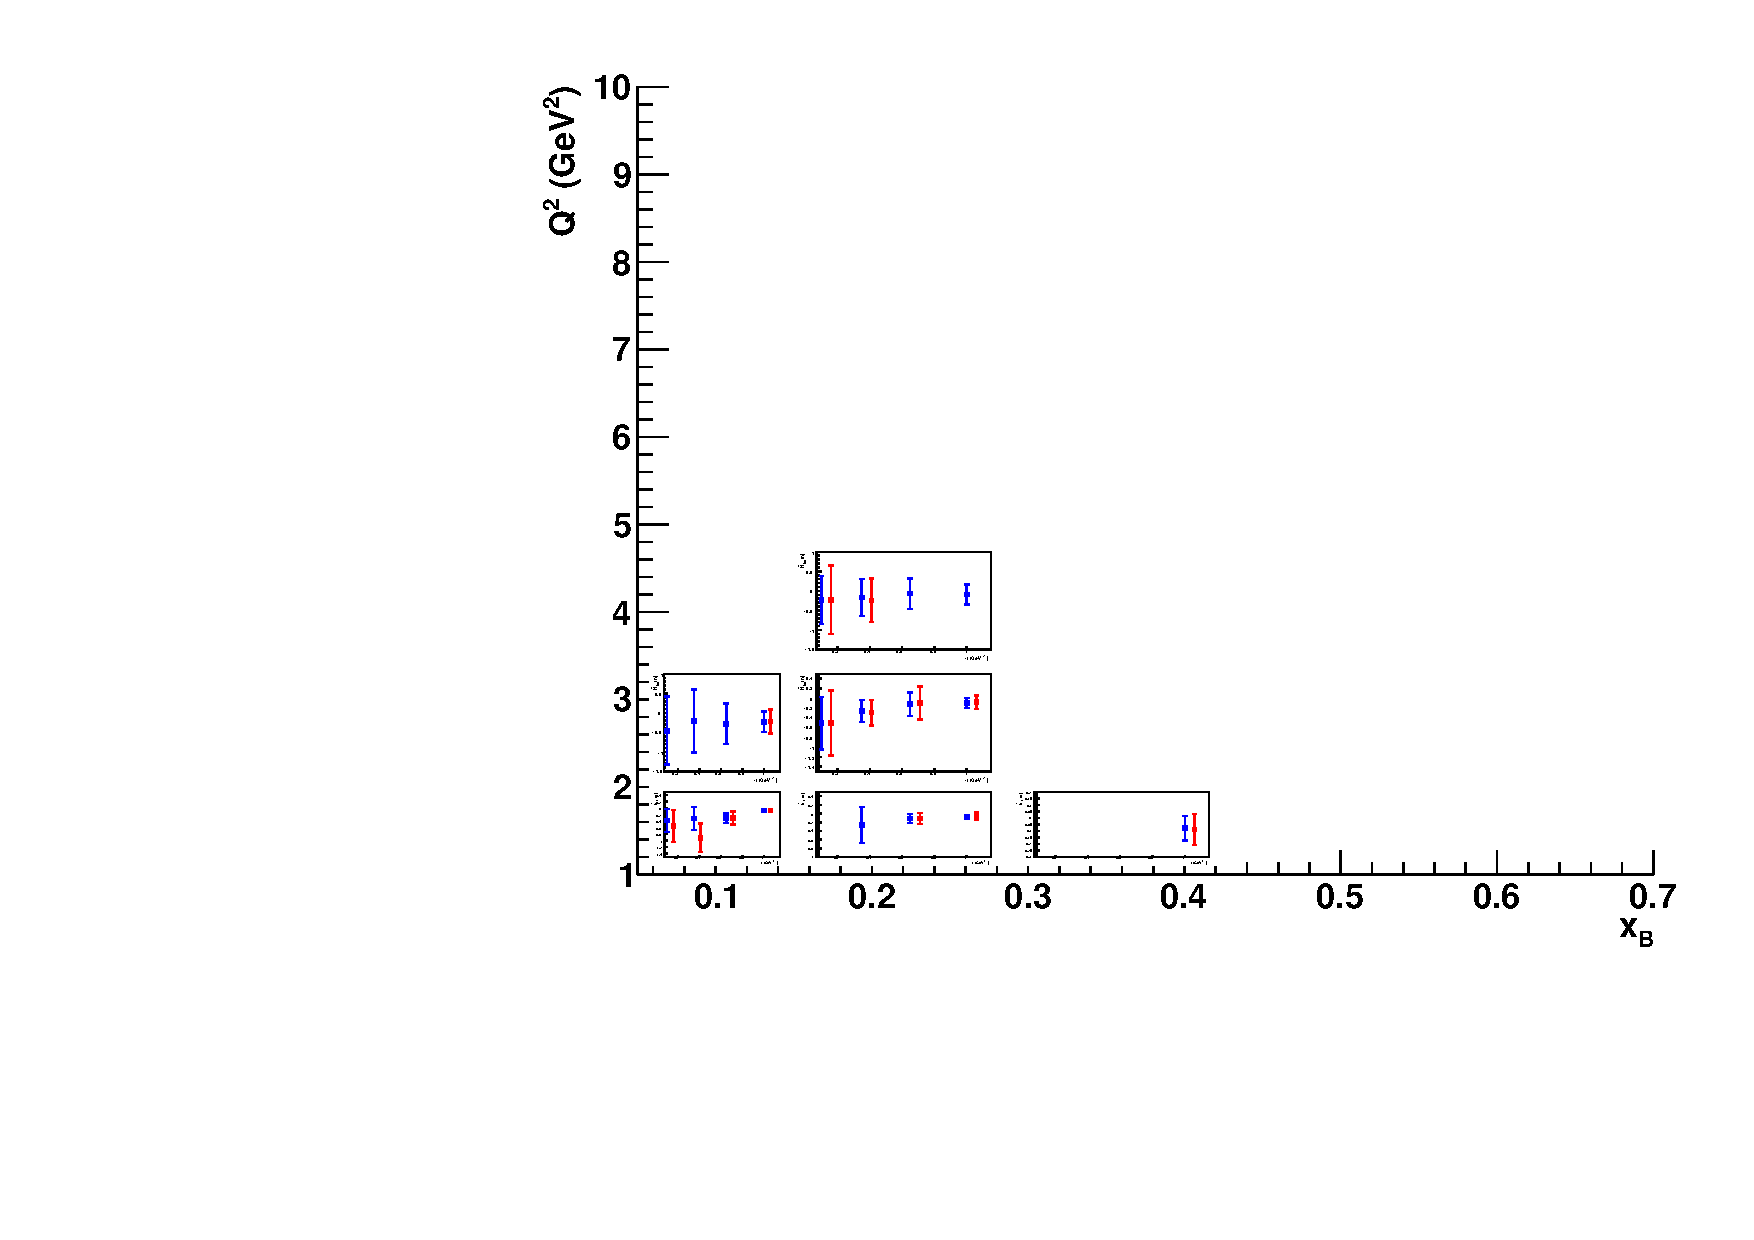
\includegraphics[width=200mm]{mixed_CFF/100/mixed/CFF_htim_compare3.pdf}
\caption[$\tilde{H}_{Im}(n)$ as a function of $-t$]
{$\tilde{H}_{Im}(n)$ as a function of $-t$, for each bin in $Q^2$ and $x_B$. The blue points are obtained with the proposed run-group extension. The red points are obtained with the existing 50 days of Run Group Cb.}\label{cff_htim}
\end{center}
\end{sidewaysfigure}

\begin{sidewaysfigure}  
\begin{center}
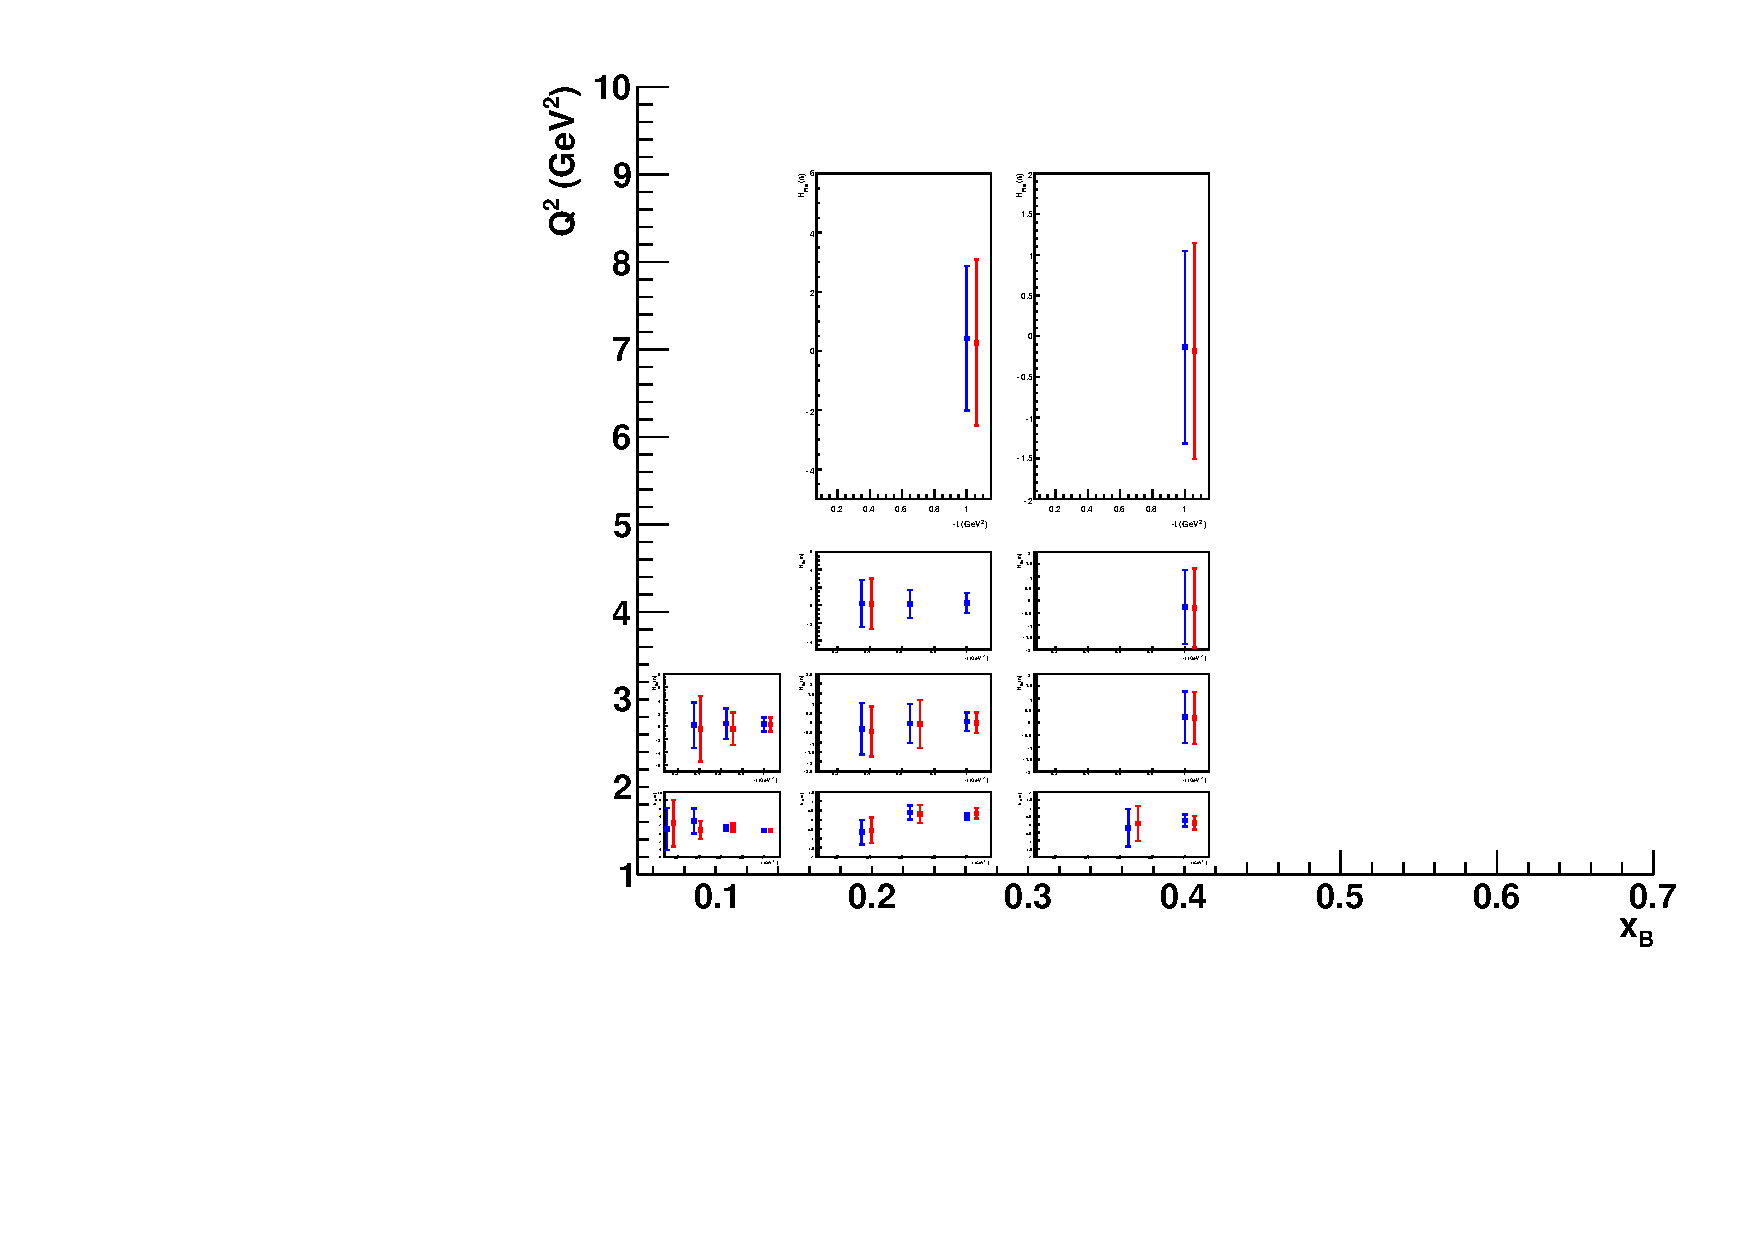
\includegraphics[width=200mm]{mixed_CFF/100/mixed/CFF_hre_compare3.pdf}
\caption[$H_{Re}(n)$ as a function of $-t$]
{$H_{Re}(n)$ as a function of $-t$, for each bin in $Q^2$ and $x_B$. The blue points are obtained with the proposed run-group extension. The red points are obtained with the existing 50 days of Run Group Cb.}\label{cff_hre}
\end{center}
\end{sidewaysfigure}

\begin{sidewaysfigure}  
\begin{center}
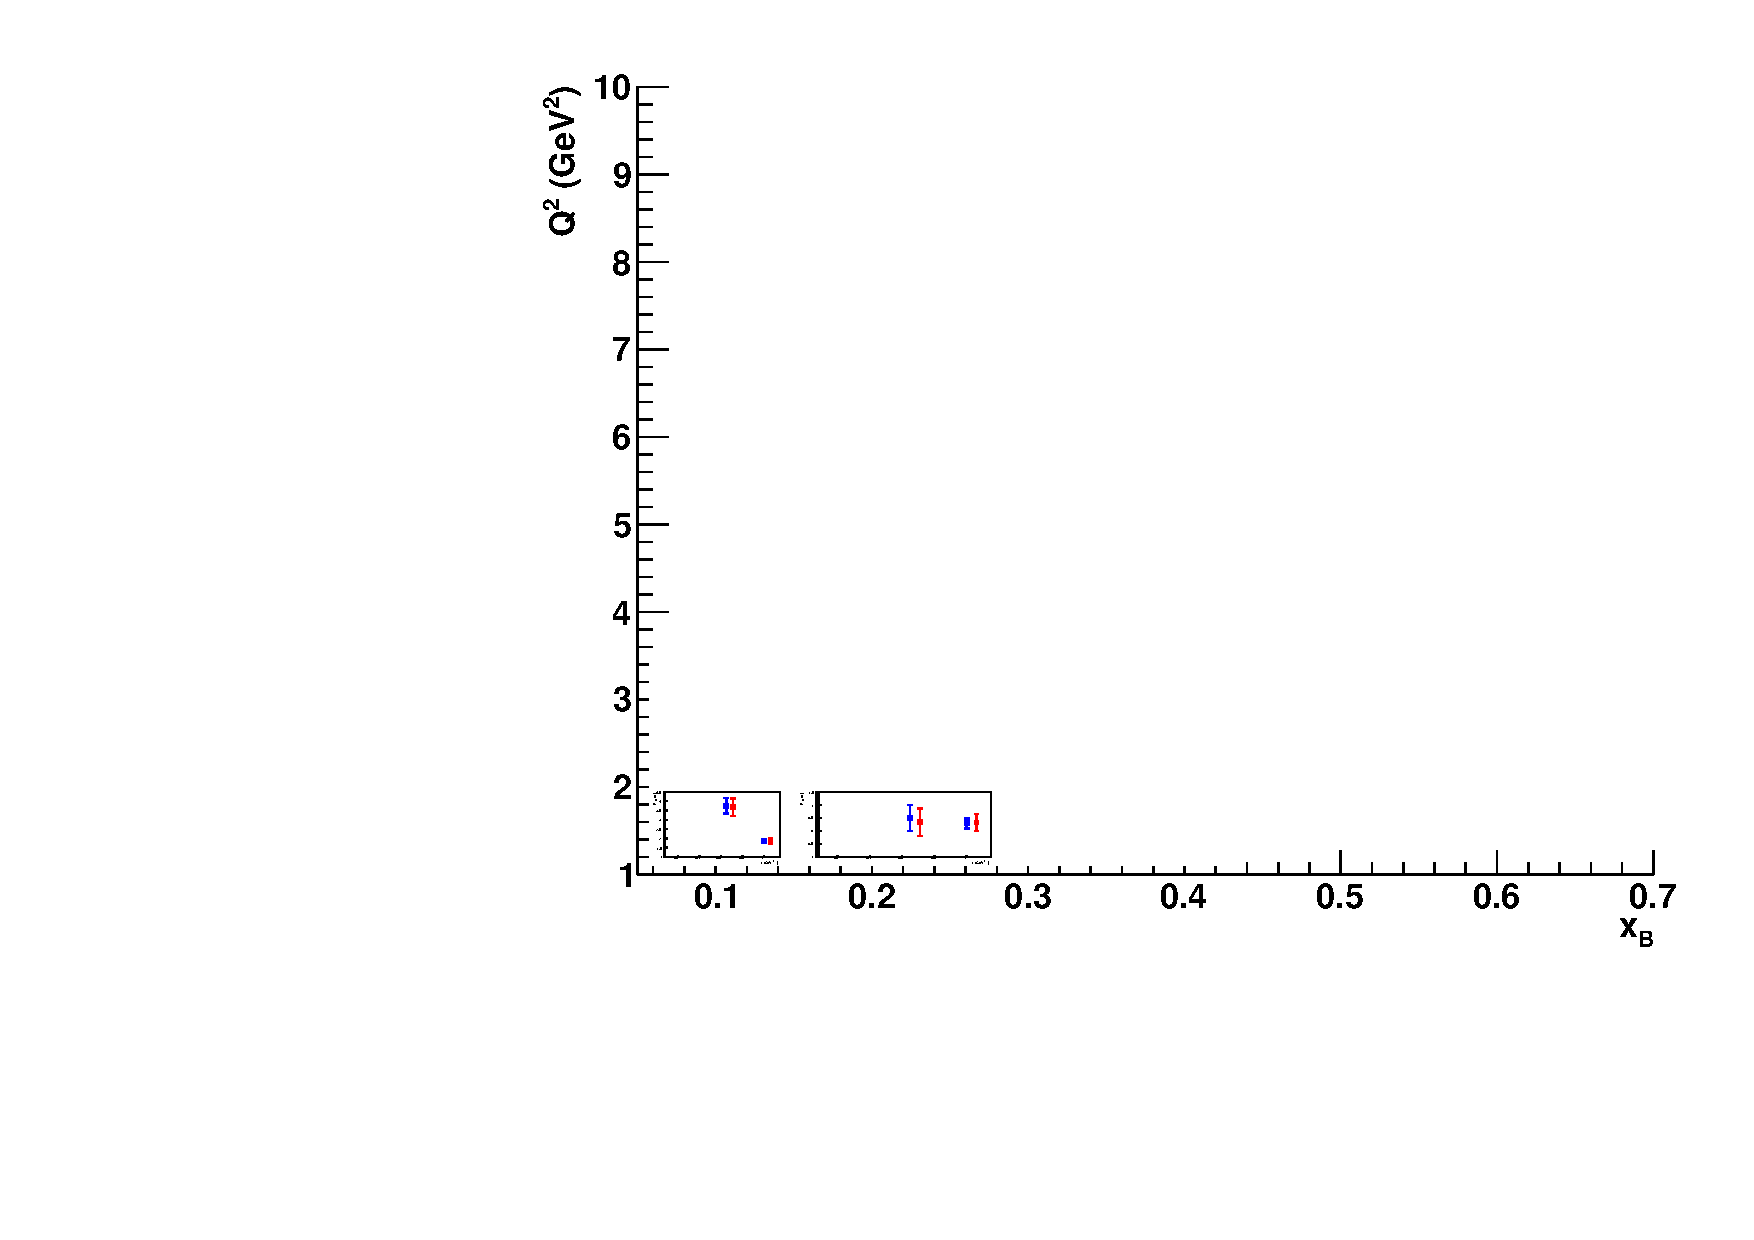
\includegraphics[width=200mm]{mixed_CFF/100/mixed/CFF_ere_compare3.pdf}
\caption[$E_{Re}(n)$ as a function of $-t$]
{$E_{Re}(n)$ as a function of $-t$, for each bin in $Q^2$ and $x_B$. The blue points are obtained with the proposed run-group extension. The red points are obtained with the existing 50 days of Run Group Cb.}\label{cff_ere}
\end{center}
\end{sidewaysfigure}

\begin{sidewaysfigure}  
\begin{center}
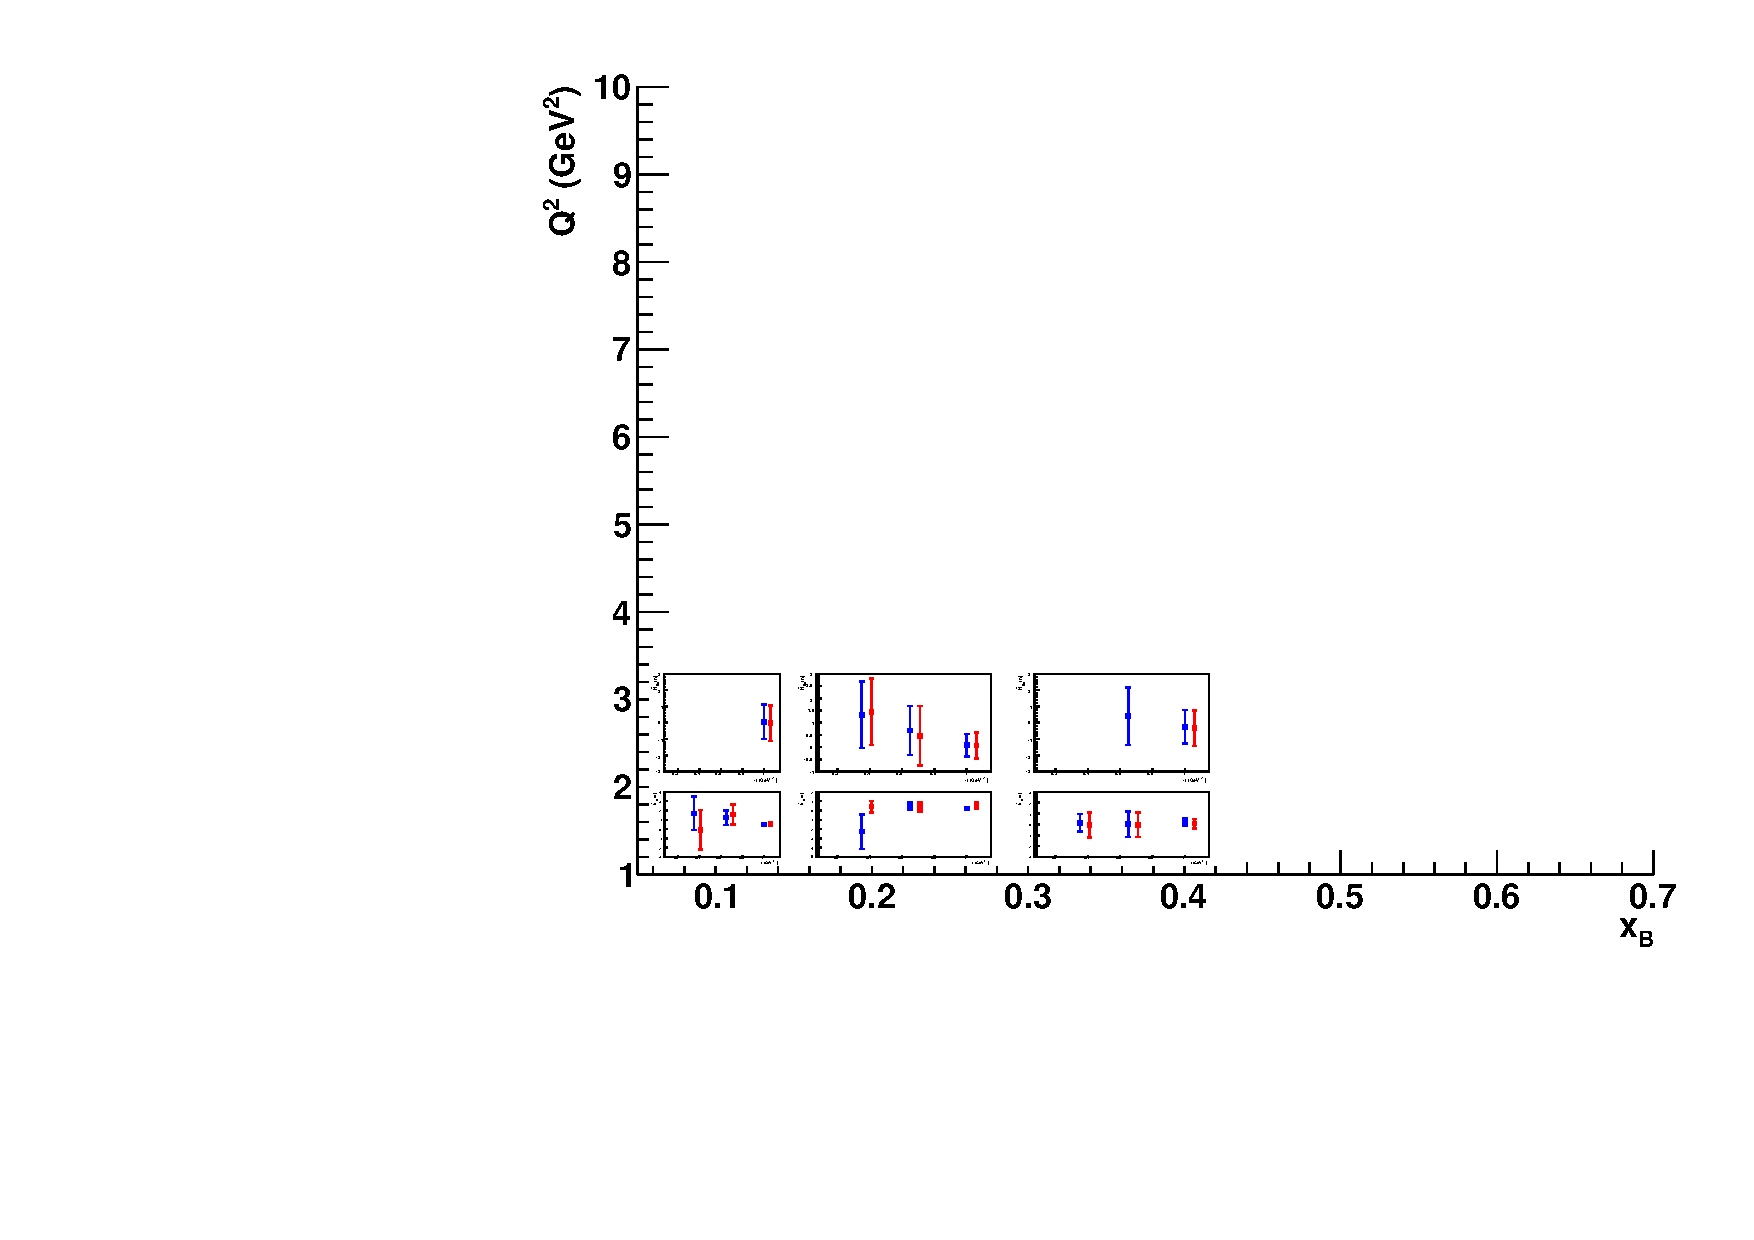
\includegraphics[width=200mm]{mixed_CFF/100/mixed/CFF_htre_compare3.pdf}
\caption[$\tilde{H}_{Re}(n)$ as a function of $-t$]
{$\tilde{H}_{Re}(n)$ as a function of $-t$, for each bin in $Q^2$ and $x_B$. The blue points are obtained with the proposed run-group extension. The red points are obtained with the existing 50 days of Run Group Cb.}\label{cff_htre}
\end{center}
\end{sidewaysfigure}

\begin{sidewaysfigure}  
\begin{center}
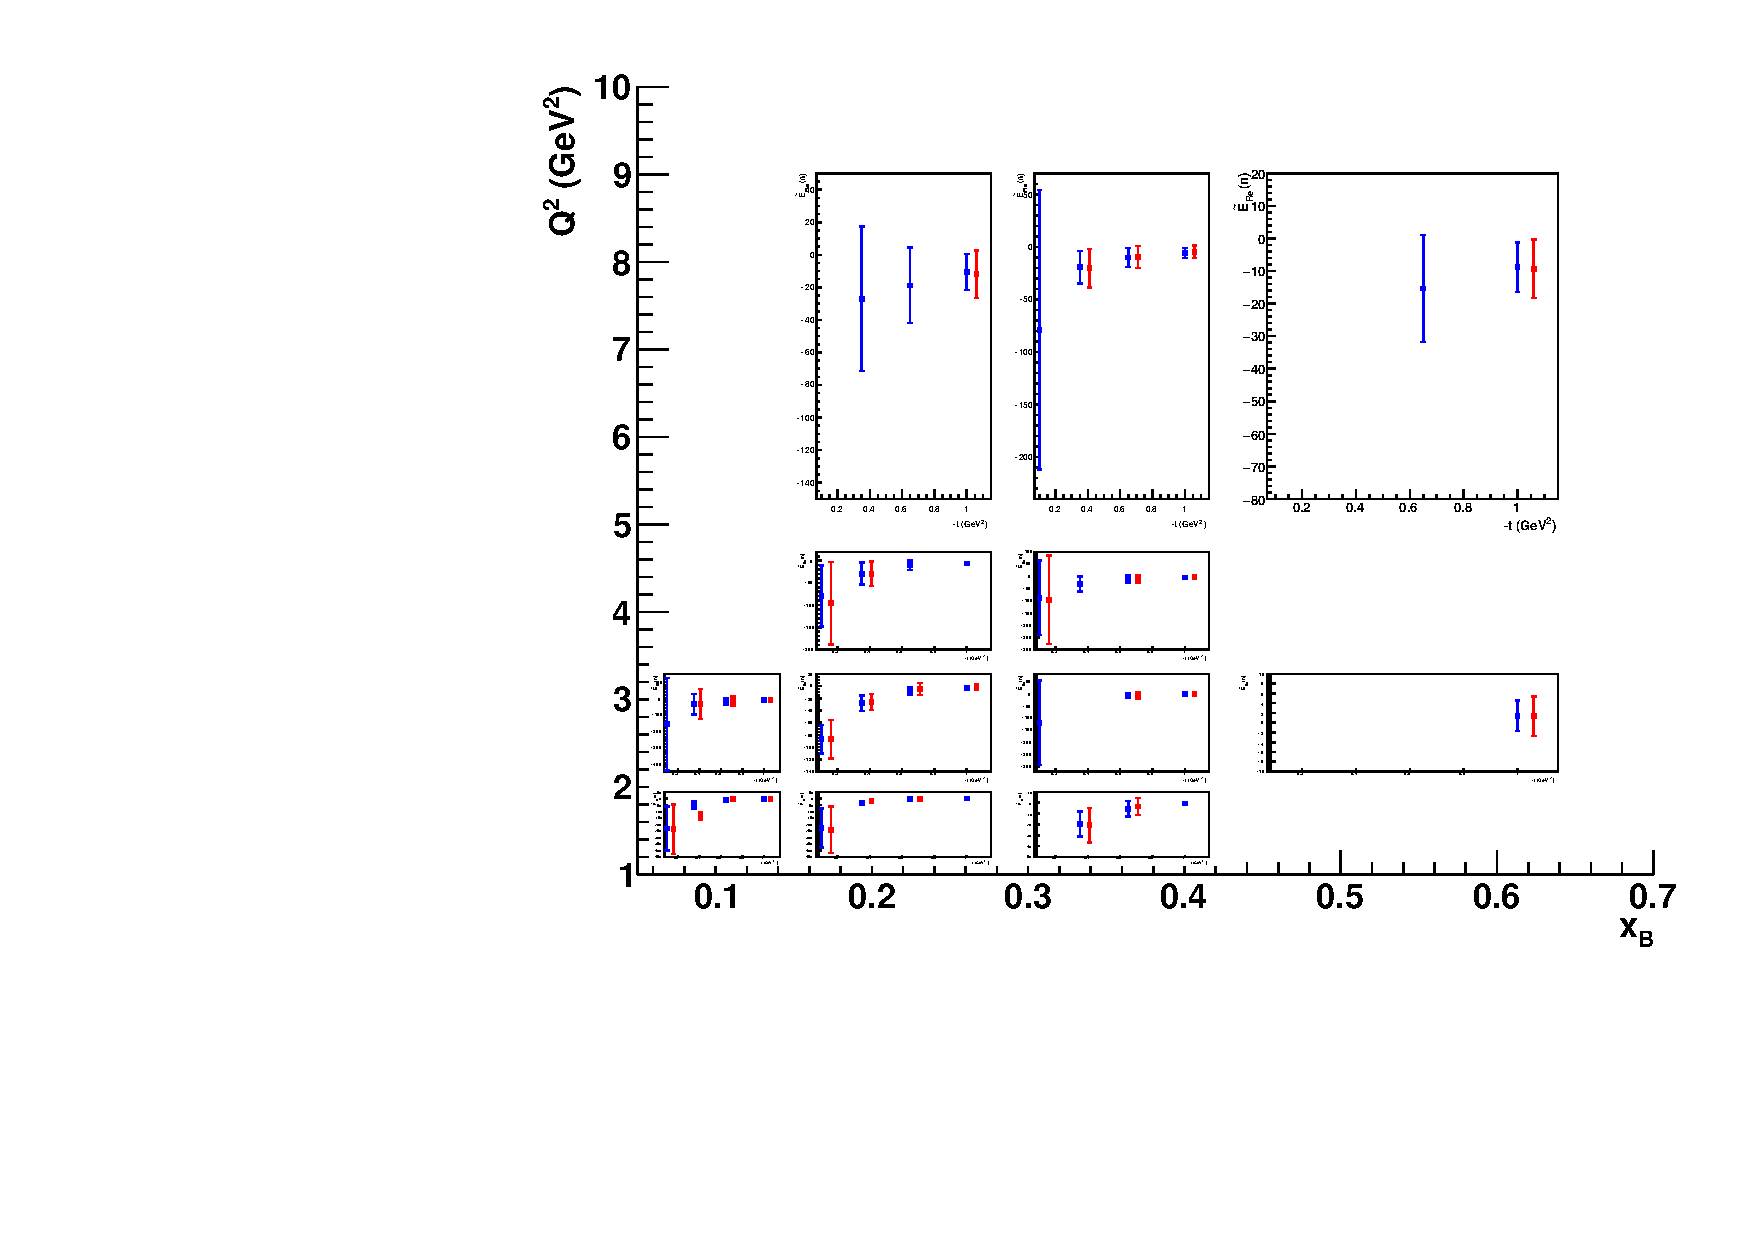
\includegraphics[width=200mm]{mixed_CFF/100/mixed/CFF_etre_compare3.pdf}
\caption[$\tilde{E}_{Re}(n)$ as a function of $-t$]
{$\tilde{E}_{Re}(n)$ as a function of $-t$, for each bin in $Q^2$ and $x_B$. The blue points are obtained with the proposed run-group extension. The red points are obtained with the existing 50 days of Run Group Cb.}\label{cff_etre}
\end{center}
\end{sidewaysfigure}

\section{Flavor separation of CFFs}
In order to convey the impact of the proposed measurement on the JLab GPD program, an example of model-independent flavor separation of CFFs, which this experiment will make possible for the first time, is shown in Figs.~\ref{flavor_h_im} and Figs.~\ref{flavor_e_im}. Here, the CFFs $H_{Im}$ (Fig.~\ref{flavor_h_im}) and $E_{Im}$ (Fig.~\ref{flavor_e_im}) are shown, for four different bins in $Q^2$-$x_B$ (left-right), as a function of $-t$, for the two nucleons (top) and for the two quark flavors (middle for $d$ and bottom for $u$). These figures has been produced using the proton CFFs that were extracted combining all the projected results for the pDVCS asymmetries that will be measured with CLAS12 \cite{mick_herve}\footnote{In the case of $E_{Im}$, the figure must be taken only as an indication of the potential of the present experiment. In fact the measurement of $E_{Im}(p)$, and its uncertainties, depend strongly on the feasibility of the conditionally approved pDVCS experiment with transversely-polarized target \cite{E1212010}.} (purple points), with the neutron CFFs that were shown in Section~\ref{sec_cff}, for the two different scenarios of beam time: the 110 days proposed in this extension request (blue points) and the existing 50 days of run group Cb (red points). 
Various observations can be made examining these figures: 
\begin{itemize}
\item{as noted before, $H_{Im}(n)$ is more sensible to variations of statistics for the ND$_3$ data than $E_{Im}(n)$, as the latter is mostly affected by the statistics of the beam-spin asymmetry; nevertheless, in some bins the impact of the extension will be important for $E_{Im}(n)$ as well. In particular, in some kinematics the fits for $E_{Im}(n)$ converge only thanks to the statistics provided by the extension;}
\item{in some kinematics, in particular at low $-t$ and low $x_B$, the presence of the Forward Tagger in the extension improves considerably the error bars or helps the fits to converge;}
\item{even with 110 days of running time on ND$_3$, the errors on neutron CFFs are much larger than those on proton ones, especially for $H$;}
\item{the uncertainty on neutron CFFs dominates the flavor-separated quark CFFs, impacting also the $u$ CFFs.}
\end{itemize}
The flavor separation of the CFFs will represent a major step forward towards the unraveling of the contribution of the quarks' angular momentum to the total nucleon spin via Ji's sum rule \cite{ji}: 
\begin{equation}
        \sum_{q}\int_{-1}^{+1}dx \, x[H^{q}(x,\xi,t=0)+E^{q}(x,\xi,t=0)]=2\, J_{quarks}.
        \label{eq_ji_rule}
\end{equation}
The low-$t$ region is very important for Ji's sum rule, and this motivates strongly the need to use the Forward Tagger to fill the gaps in the CLAS12 acceptance at such kinematics. 

\begin{figure}  
\begin{center}
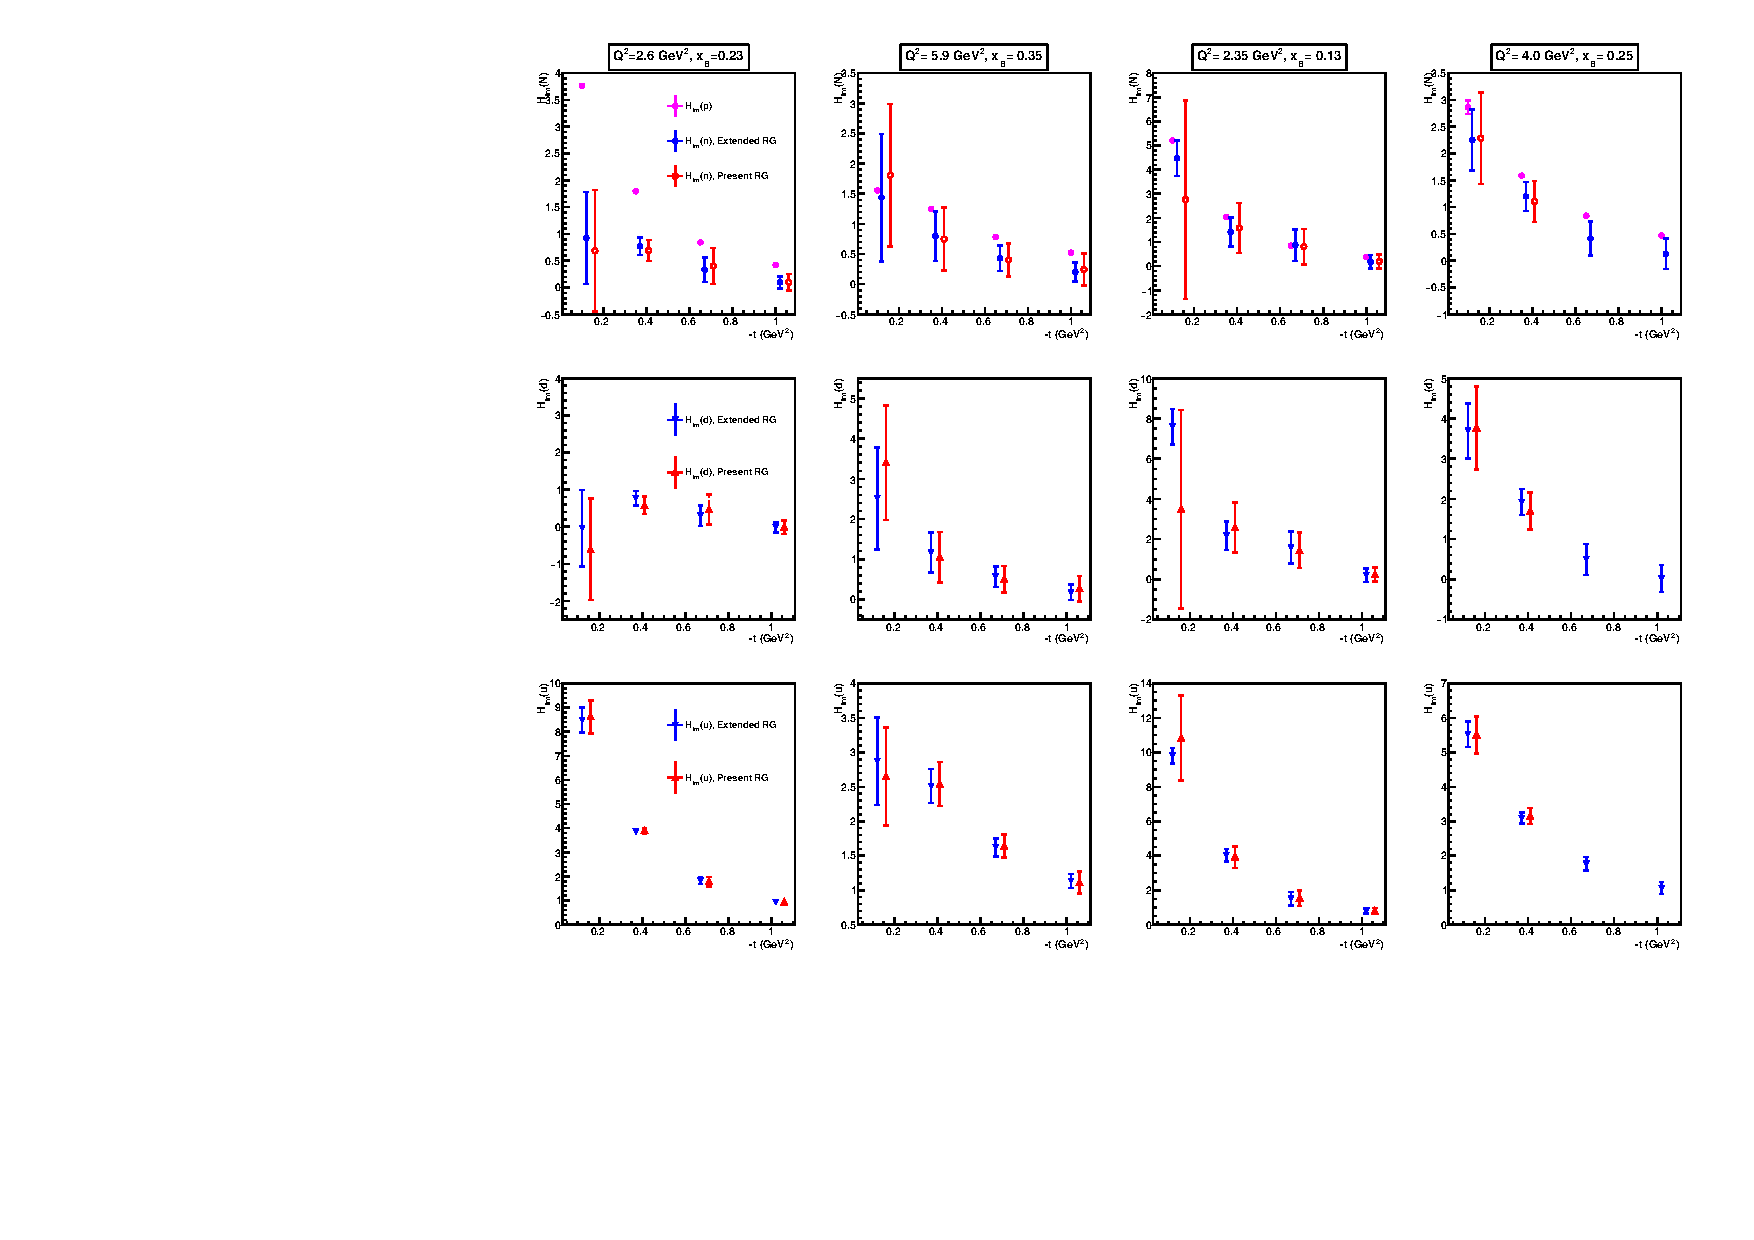
\includegraphics[width=160mm]{flavors_h_im_compare3.pdf}
\caption[Flavor separation of the $H_{Im}$ CFF]
{Top: ${H}_{Im}(p)$ (purple), extracted from the projections for the approved and conditionally-approved proton-DVCS CLAS12 experiments, and ${H}_{Im}(n)$, obtained from the projections of the proposed experiment extension (blue) and from the projections for the already approved 50 days of run-group Cb (red), as a function of $-t$. The middle and bottom lines show the quark-flavor separated ${H}_{Im}$, for $d$ and for $u$ quarks, respectively. Four different bins in $Q^2$-$x_B$, indicated in the legends, are shown in the four columns.}\label{flavor_h_im}
\end{center}
\end{figure}

\begin{figure}  
\begin{center}
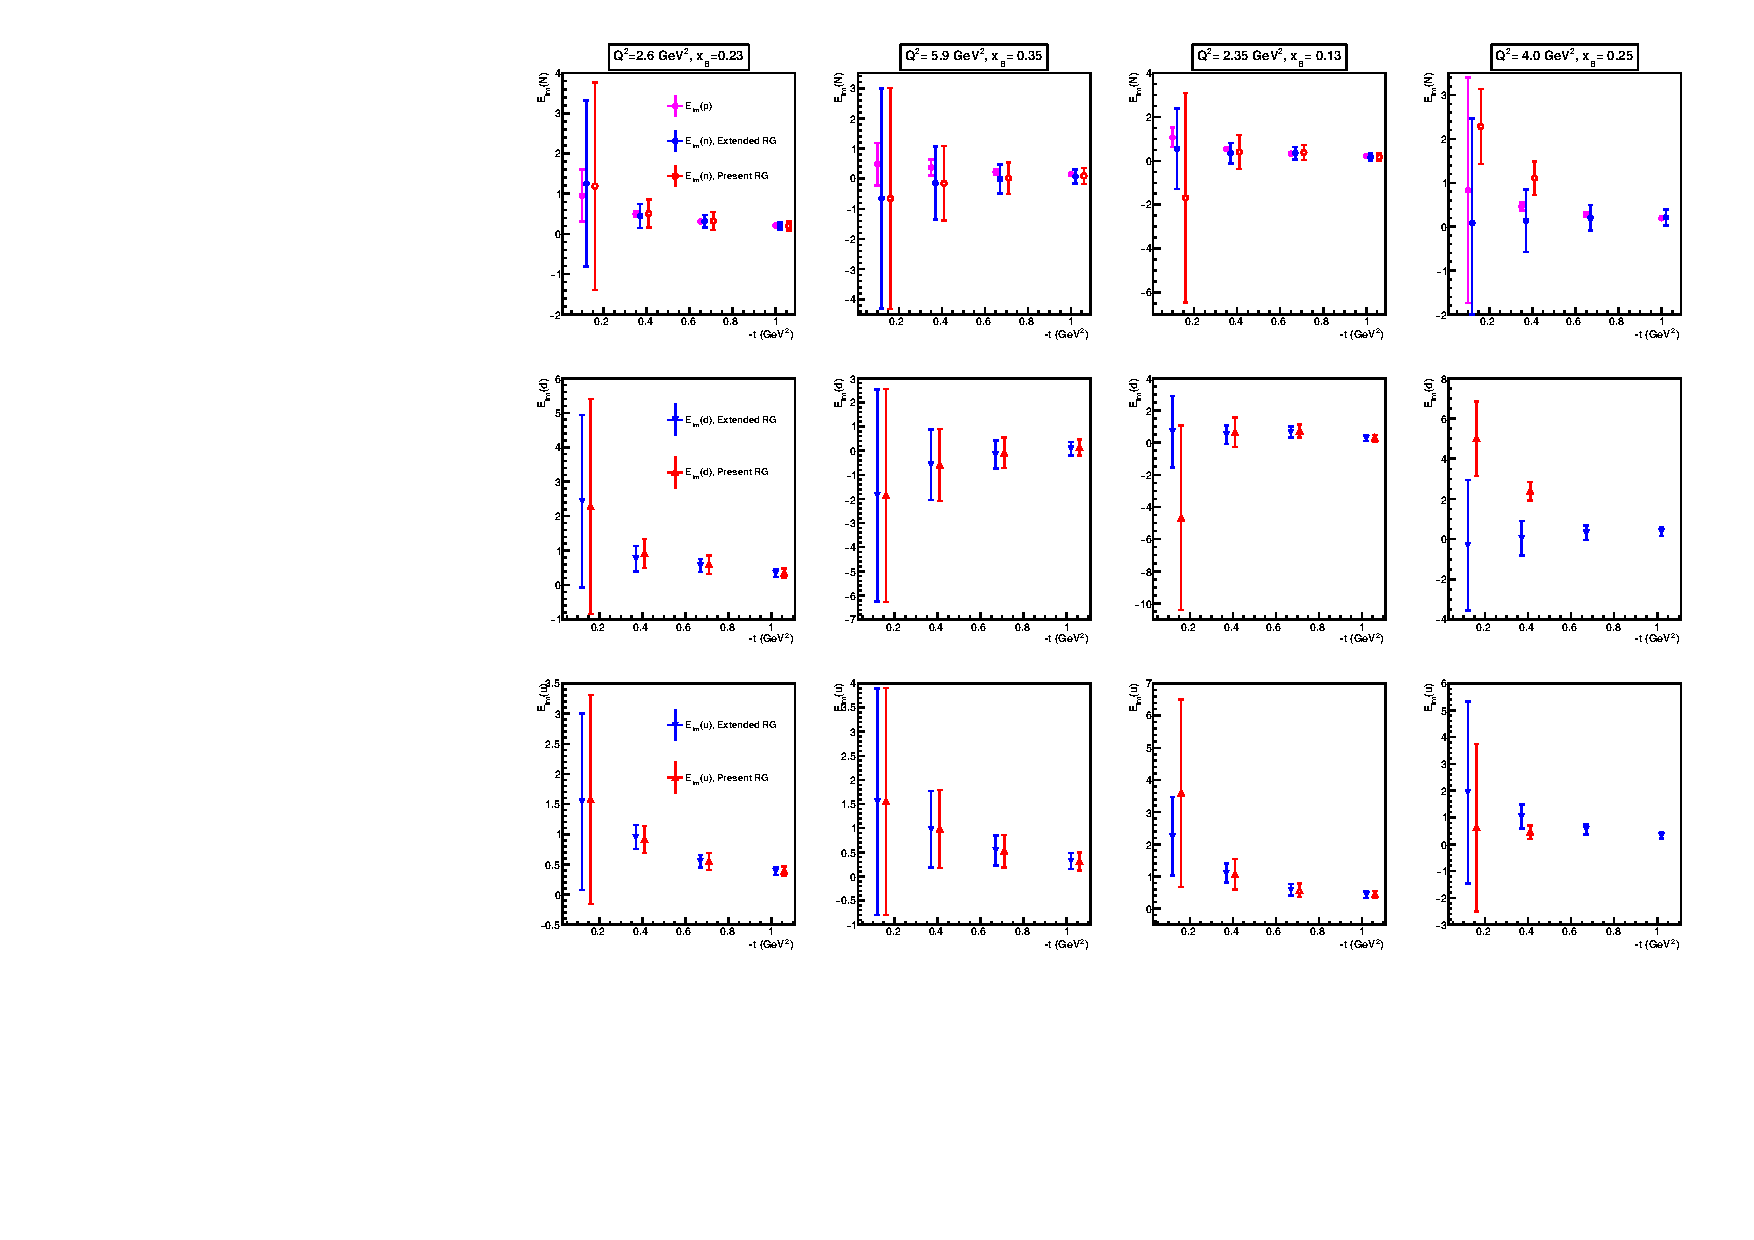
\includegraphics[width=160mm]{flavors_e_im_compare3.pdf}
\caption[Flavor separation of the $E_{Im}$ CFF]
{Top: ${E}_{Im}(p)$ (purple), extracted from the projections for the approved and conditionally-approved proton-DVCS CLAS12 experiments, and ${E}_{Im}(n)$, obtained from the projections of the proposed experiment extension (blue) and from the projections for the already approved 50 days of run-group Cb (red), as a function of $-t$. The middle and bottom lines show the quark-flavor separated ${E}_{Im}$, for $d$ and for $u$ quarks, respectively. Four different bins in $Q^2$-$x_B$, indicated in the legends, are shown in the four columns.}\label{flavor_e_im}
\end{center}
\end{figure}
